\subsubsection{Design af elementer}
Herunder vil designet af en stor del af Kommunikationen i grænsefladen blive beskrevet, først med klassediagrammer og derefter med sekvensdiagrammer.\\

\textbf{Klassediagrammer}\\

\begin{figure}[H]
	\centering
	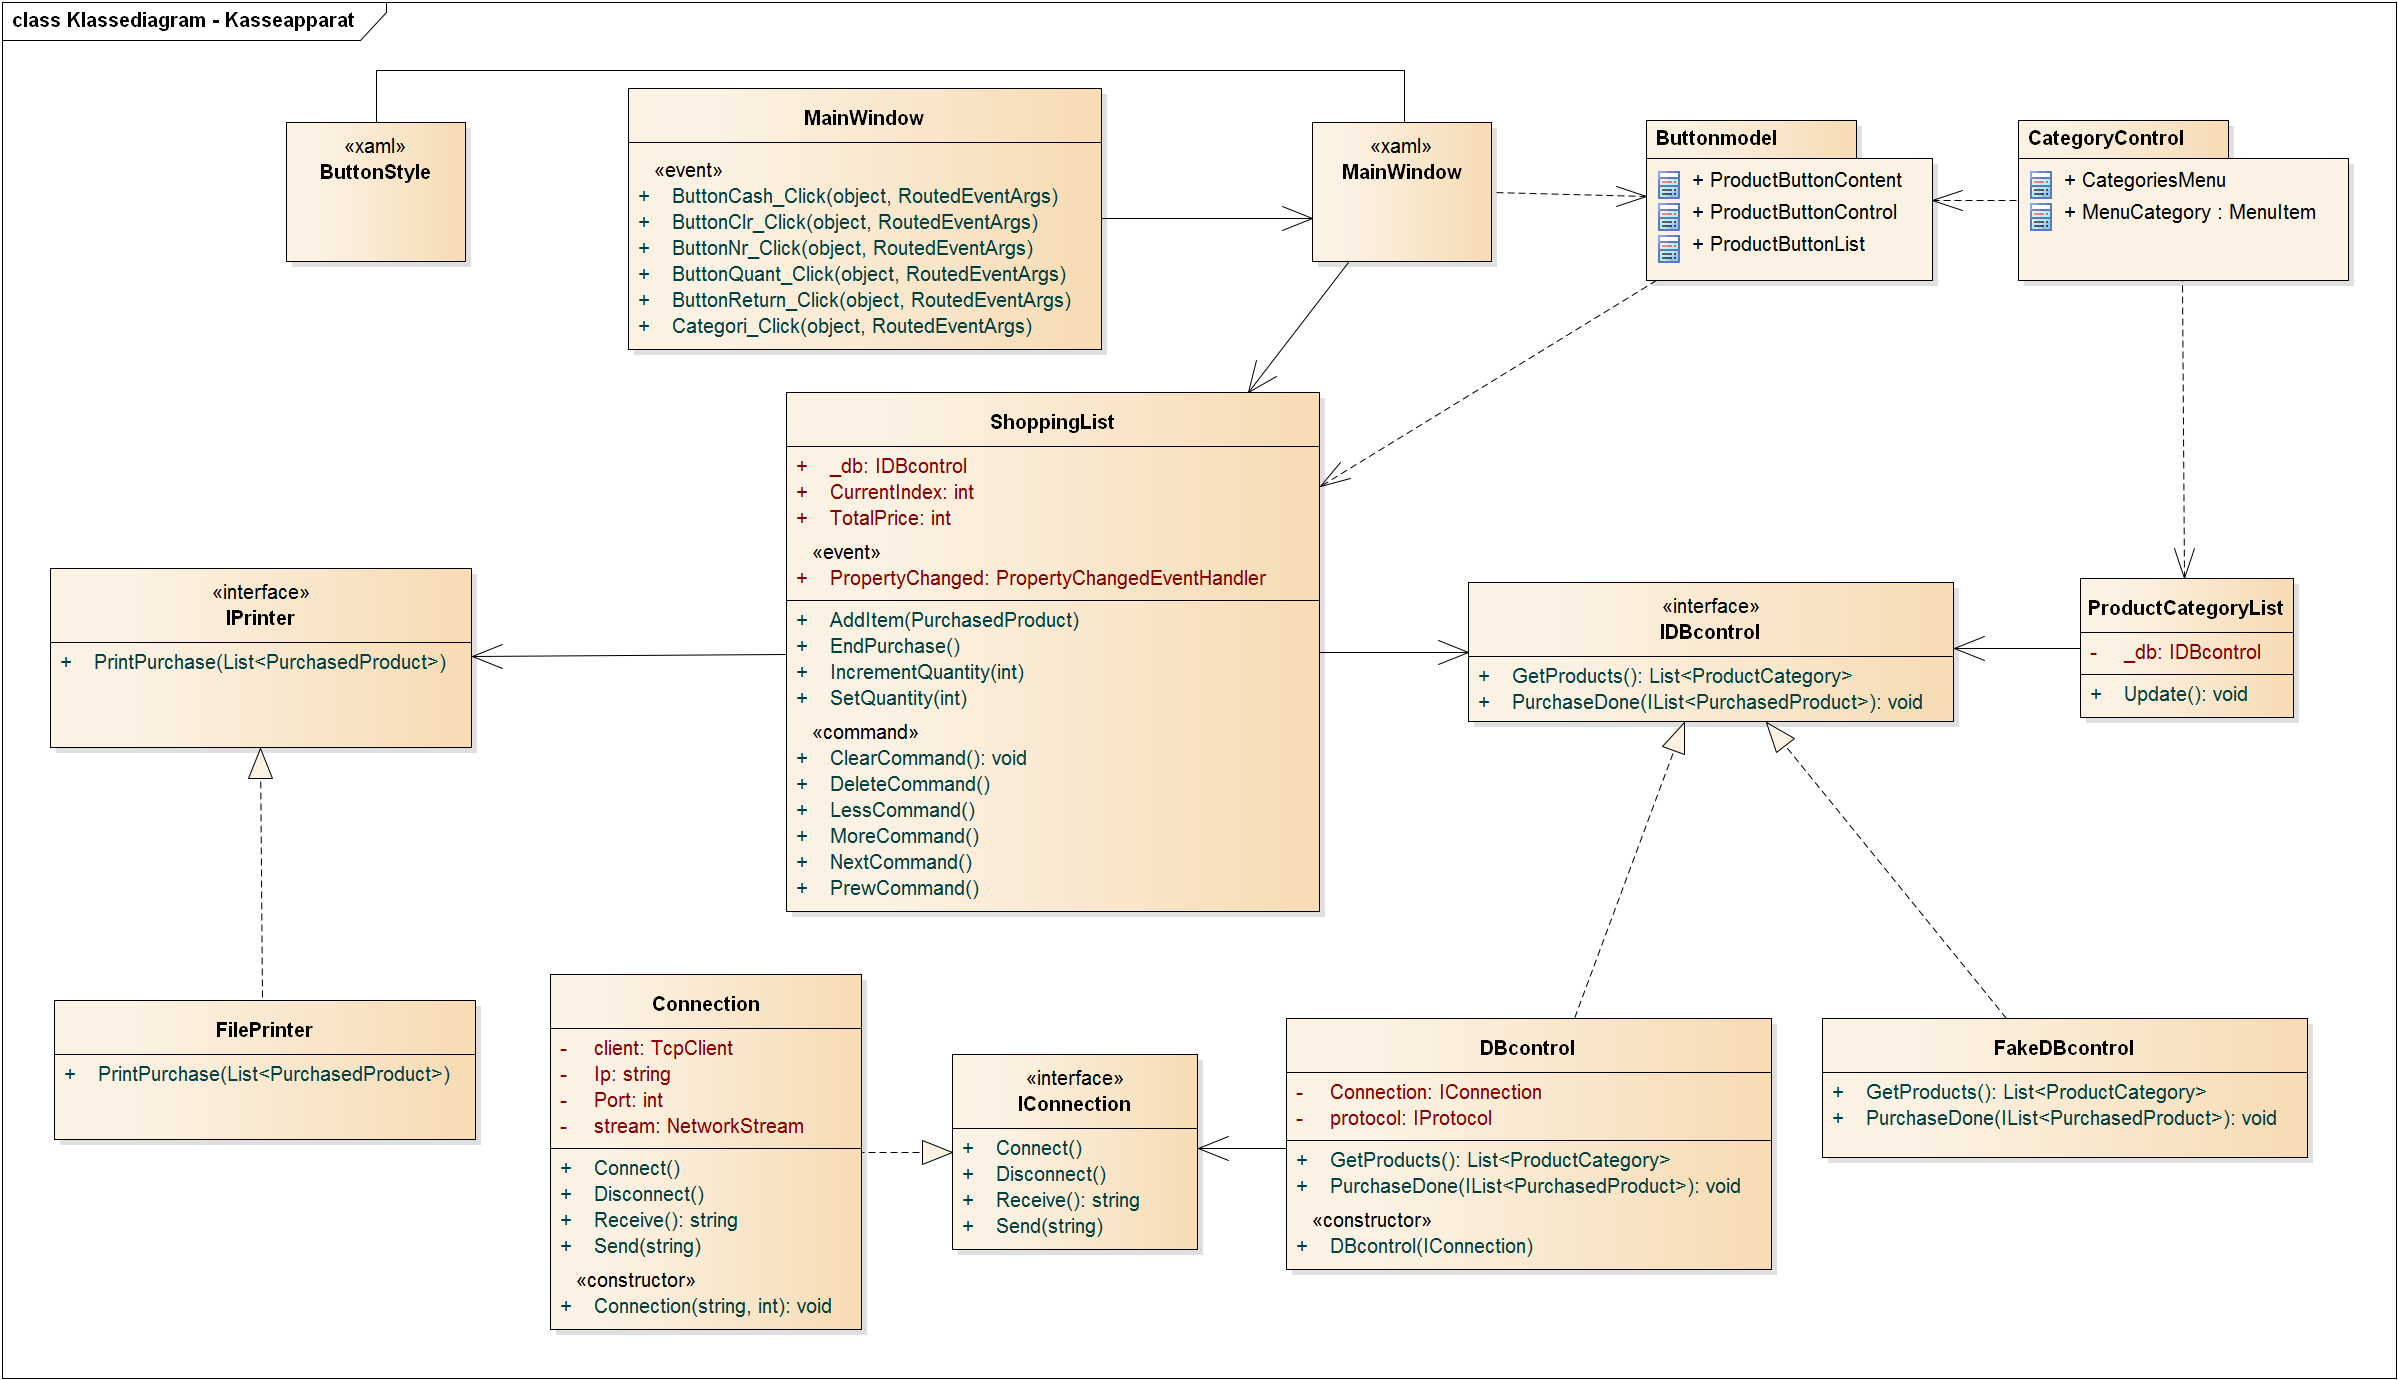
\includegraphics[width=1.2\textwidth, angle=90]{Systemdesign/Frontend/GUI/DesignOgStruktur/Pics/KlassediagramKasseApparat}
	\caption{Klassediagram over kasseapparat.}
	\label{fig:KasseKlasse}
\end{figure}

På figur \ref{fig:KasseKlasse} kan man se hele kasseapparatets software vist ved dens klasser og funktioner. Dog er ViewModels delt op i 2 pakker. Dette er bestemt, da det ville give mere mening at gøre det på denne måde når man skulle forklare klasserne og deres indbyrdes forhold. \\
Klassediagrammet er delt op i 3 lag, der skal symbolisere henholdsvis Præsentationslag, Business logic og Data access

\begin{figure}[H]
	\centering
	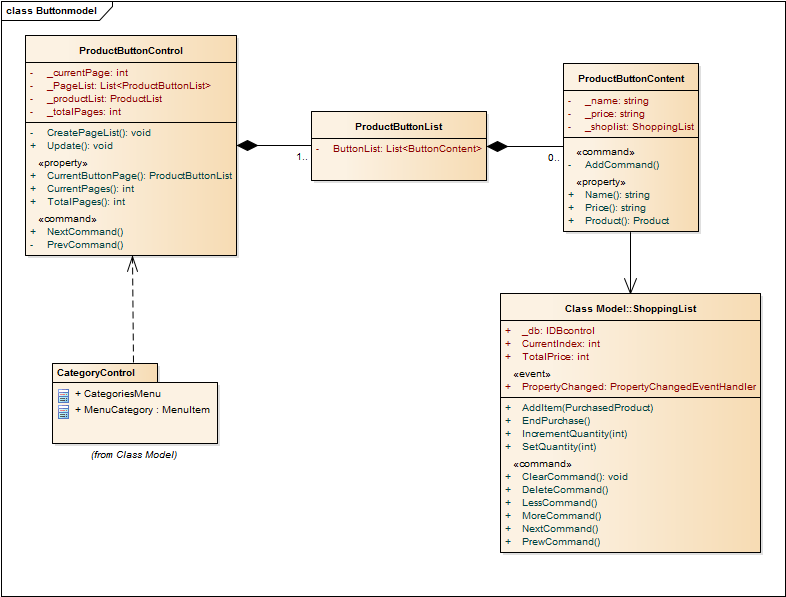
\includegraphics[width=1\textwidth]{Systemdesign/Frontend/GUI/DesignOgStruktur/Pics/KlassediagramButtonModel}
	\caption{Klassediagram over ViewModel pakken ButtonModel.}
	\label{fig:EndeligeGUI}
\end{figure}

\begin{figure}[H]
	\centering
	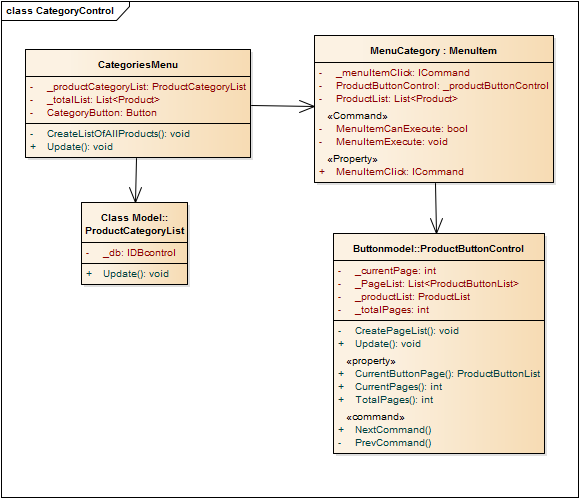
\includegraphics[width=1\textwidth]{Systemdesign/Frontend/GUI/DesignOgStruktur/Pics/KlassediagramCategoryControl}
	\caption{Pakkediagram over ViewModel pakken CategoryControl.}
	\label{fig:EndeligeGUI}
\end{figure}